% LED Flasher PCB Design, Eclectronics Fall 2026
% Build: latexmk report.tex (PDF here, aux files in build/)
\documentclass[11pt]{article}

\usepackage[margin=0.5in]{geometry}
\usepackage[T1]{fontenc}
\usepackage{cmbright}
\usepackage{microtype}
\usepackage{parskip}

\usepackage{amsmath}
\usepackage{siunitx}
\sisetup{
  per-mode = symbol,
  range-phrase = --,
  range-units = single,
  retain-explicit-plus = true,
}

\usepackage{graphicx}
\graphicspath{{figures/}}
\usepackage{booktabs}
\usepackage{array}
\usepackage{tabularx}
\usepackage{caption}
\captionsetup{font=small, labelfont=bf}
\usepackage{float}
\usepackage{enumitem}
\setlist{nosep}
\usepackage[hidelinks]{hyperref}
\usepackage{cleveref}

\newcommand{\Vdd}{V_{\text{DD}}}
\newcommand{\Vth}{V_{\text{TH}}}
\newcommand{\Vtl}{V_{\text{TL}}}

\begin{document}
\begin{center}
  {\LARGE\bfseries LED Flasher PCB Design}\\[3pt]
  {\large Eclectronics Fall 2026 at Olin College}\\[2pt]
  David Barsoum
\end{center}
\vspace{4pt}

\section{Overview}
The goal of this assignment is to design a small LED-flasher PCB as the
kickoff project for the Eclectronics course and to get up to speed on the
board-design tools (KiCad and LTspice) used for the rest of the semester.
The board runs off a USB type-A port and flashes an LED at \qty{1}{\Hz},
within $\pm\qty{10}{\percent}$.

The allowed parts list contains no clock or timer IC, so the oscillation
has to come from resistors, capacitors, and an op-amp. The result is a
hysteretic (Schmitt-trigger) relaxation oscillator. \Cref{fig:board}
shows the finished board layout; the schematic is in \cref{fig:schematic}.

\begin{figure}[H]
  \centering
  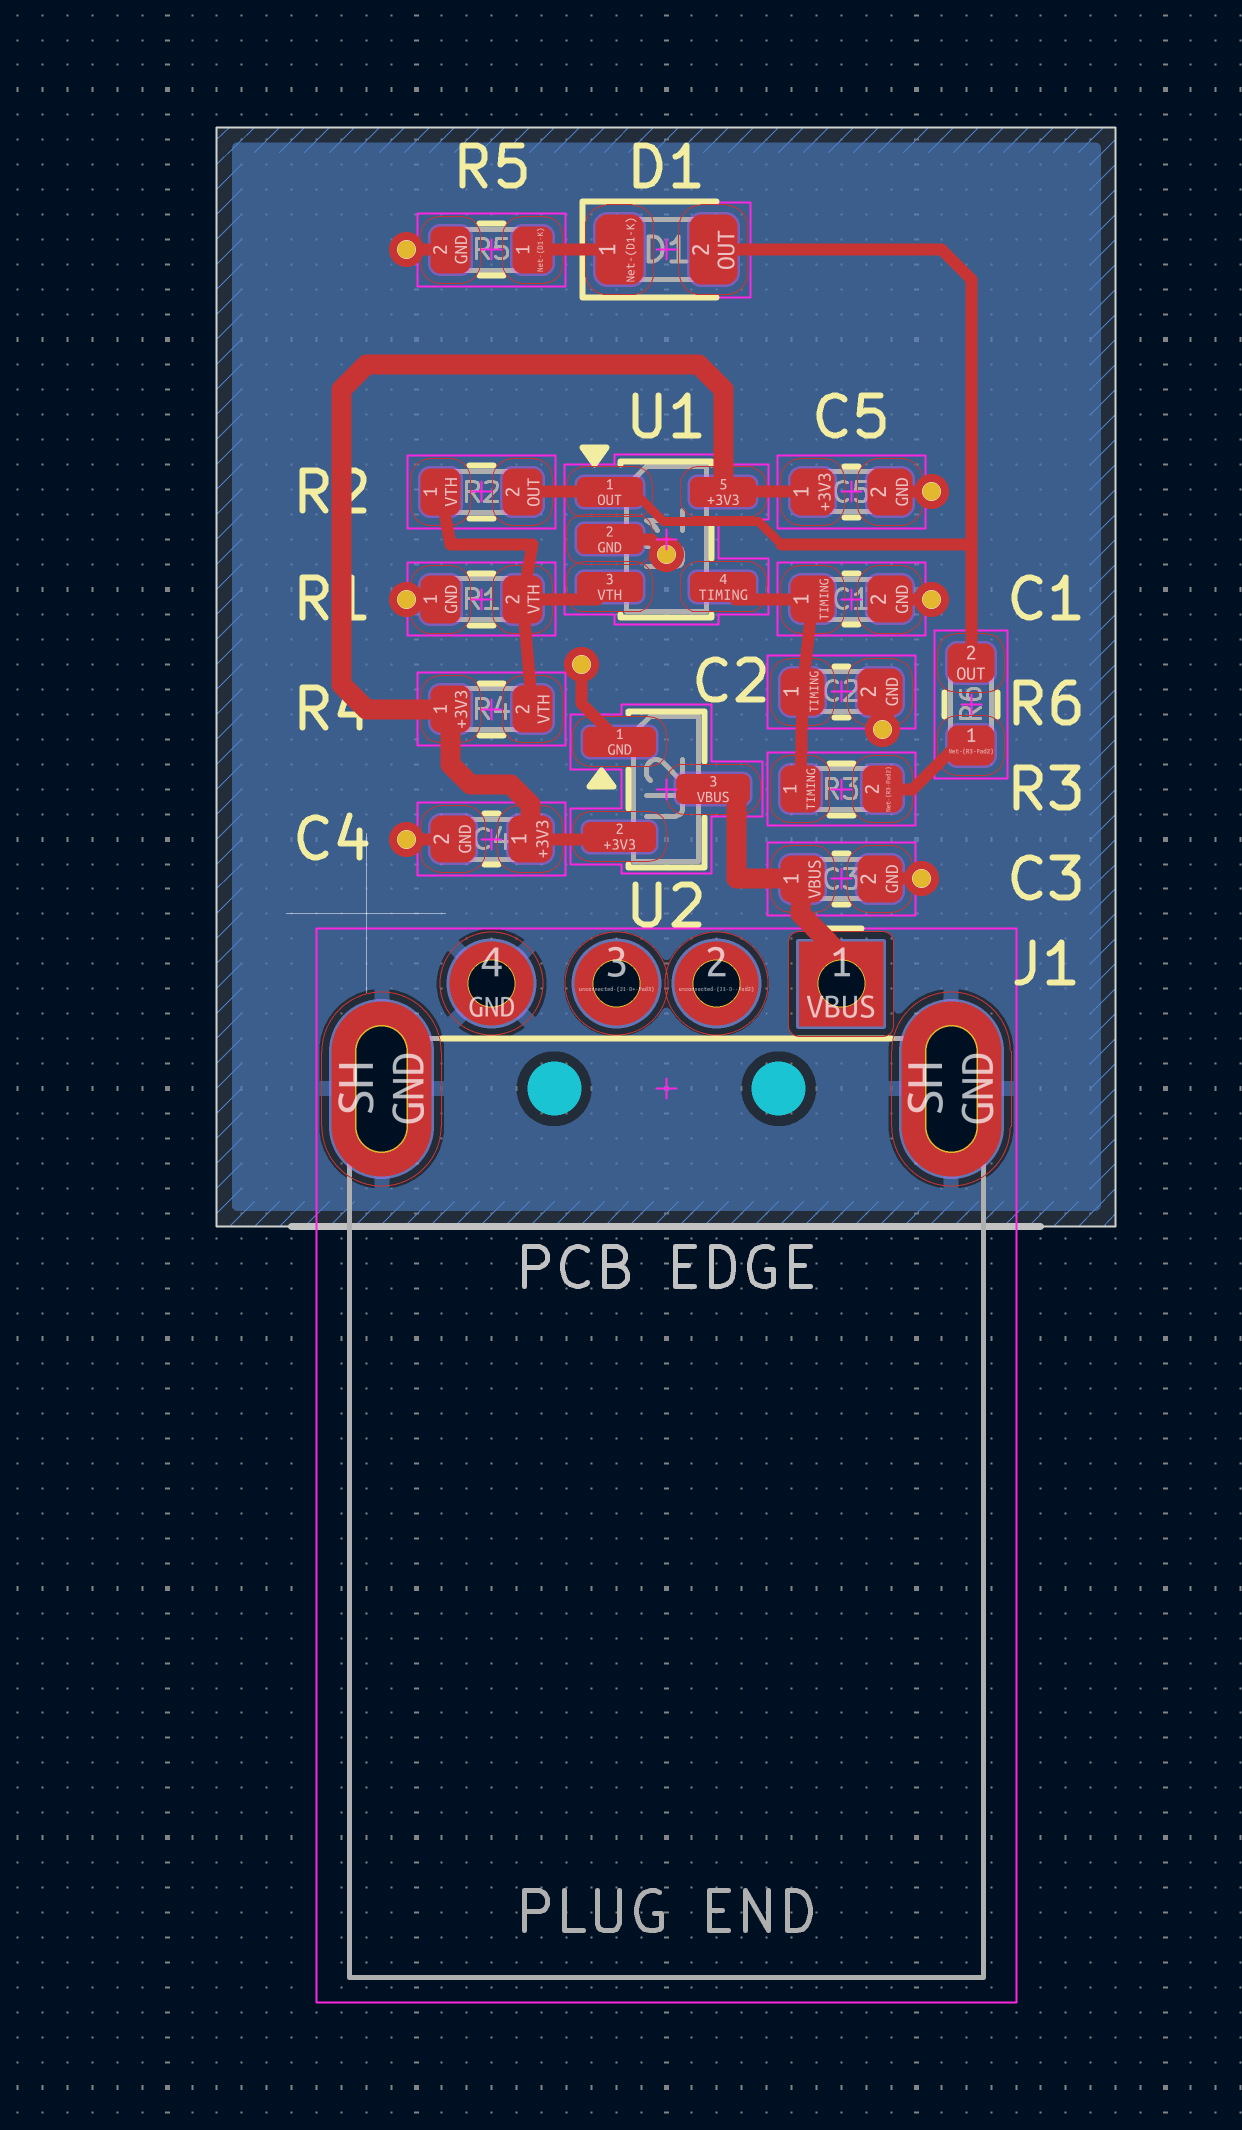
\includegraphics[angle=90, width=0.97\linewidth]{pcb-editor.png}
  \caption{PCB layout in the KiCad editor, with the USB plug end to the
  right.}
  \label{fig:board}
\end{figure}

\subsection{Requirements summary}
\begin{enumerate}[itemsep=4pt]
  \item \textbf{Flash period of \qty{1}{\s} $\pm$ \qty{10}{\percent}.}
        The nominal design is \qty{1.002}{\s}. \Cref{sec:tolerance} shows
        the worst-case period over component tolerances is
        \qtyrange{0.929}{1.078}{\s}, within the window.

  \item \textbf{Single-ended \qty{3.3}{\volt} supply from USB
        \qty{5}{\volt} VBUS.} An MCP1702-3302 linear regulator steps VBUS
        down to \qty{3.3}{\volt}.

  \item \textbf{Components only from the provided spreadsheet.} Every part
        in the BoM (\cref{sec:bom}) is from the course list.

  \item \textbf{Adequate bypass and bulk capacitance.} Bulk capacitors on
        the regulator keep it stable and hold the rail steady; a bypass
        capacitor at the op-amp supply pin keeps switching noise off the
        rail so it cannot jitter the oscillator thresholds.

  \item \textbf{Two-layer PCB, all components on top, 6-mil trace/space,
        24-mil vias with 12-mil drills, no vias in pads.} These constraints
        keep the board simple and cheap to build.
\end{enumerate}

\section{Circuit Design}
\begin{figure}[H]
  \centering
  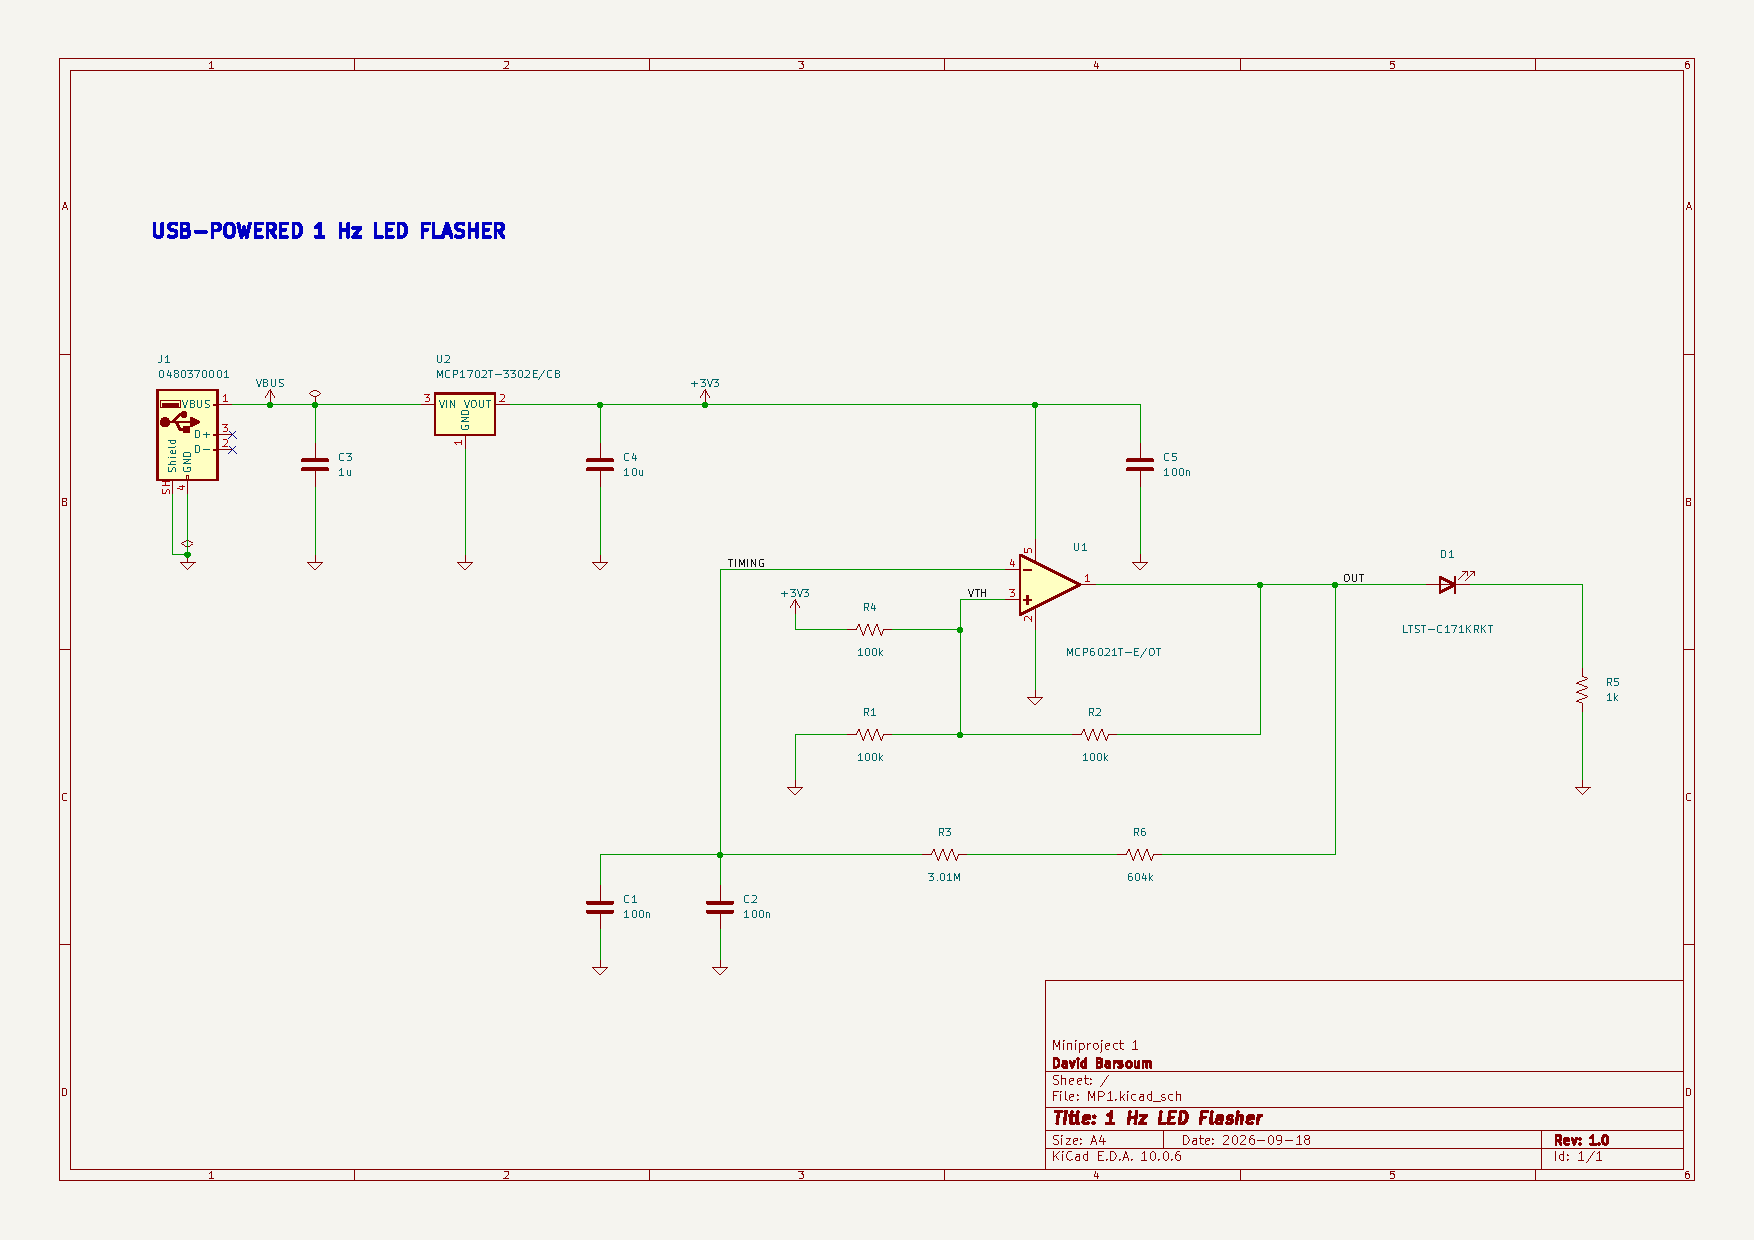
\includegraphics[width=\linewidth, trim=20mm 40mm 18mm 32mm, clip]{Schematic.pdf}
  \caption{Full circuit schematic (KiCad).}
  \label{fig:schematic}
\end{figure}

\subsection{Oscillator}
\label{sec:osc}
The oscillator can be thought of as built up in three steps:
\begin{enumerate}[itemsep=4pt]
\item \textbf{Comparator.}
An op-amp with no feedback is a comparator: its huge open-loop gain drives
the output to one rail or the other depending on which input is higher.
With a rail-to-rail part on a \qty{3.3}{\volt} supply the output is either
$\approx 0$ or $\approx\Vdd$. The problem is that there is only one
threshold, so a signal near it makes the output chatter on any noise.

\item \textbf{Schmitt trigger.}
Adding positive feedback (a resistor from the output to the non-inverting
input) makes the threshold depend on the current output state. When the
output is high the threshold is $\Vth$; when it is low the threshold drops
to $\Vtl$. The circuit remembers its last state, and the gap between the
two thresholds is the hysteresis.

\item \textbf{Relaxation oscillator.}
Adding negative feedback through a resistor $R$ to a capacitor $C$ on the
inverting input turns the Schmitt trigger into an oscillator. When the
output is high, $C$ charges through $R$ toward $\Vdd$. Once it crosses $\Vth$ the output flips low, the current reverses,
and $C$ discharges toward ground. When it falls below $\Vtl$ the output
flips high again. The result is a square wave, which drives the LED.
\end{enumerate}

\paragraph{Period and duty cycle.}
Each half of the cycle is the capacitor charging or discharging through
$R$ between the two thresholds, so
\begin{equation}
  t_{\text{high}} = RC\,\ln\!\left(\frac{\Vdd-\Vtl}{\Vdd-\Vth}\right), \qquad
  t_{\text{low}}  = RC\,\ln\!\left(\frac{\Vth}{\Vtl}\right), \qquad
  T = t_{\text{high}} + t_{\text{low}}.
  \label{eq:halves}
\end{equation}
$R$ and $C$ appear the same way in both halves, so they set how long the
period is but not the duty cycle. The duty cycle comes from where the
thresholds sit: if they are evenly spaced around the middle of the supply,
the two halves take the same time.

In this design the three threshold resistors are all \qty{100}{\kilo\ohm},
so the non-inverting input sits at the average of $\Vdd$, ground, and the
output. That gives
\begin{equation}
  \Vth = \tfrac{2}{3}\Vdd = \qty{2.20}{\volt}, \qquad
  \Vtl = \tfrac{1}{3}\Vdd = \qty{1.10}{\volt},
  \label{eq:thresholds}
\end{equation}
which are evenly spaced around $\Vdd/2$, so the duty cycle is
\qty{50}{\percent} and both logarithms in \cref{eq:halves} reduce to
$\ln 2$:
\begin{equation}
  T = 2RC\ln 2 .
  \label{eq:Tsimple}
\end{equation}
$\Vdd$ drops out, so the period does not depend on the exact supply
voltage.

\subsection{Power supply}
\label{sec:power}
The USB connector supplies \qty{5}{\volt} on VBUS, and the circuit needs
\qty{3.3}{\volt}, so an MCP1702-3302 linear regulator steps it down. A
linear regulator is appropriate because the load is only a few
milliamps, so the \qty{1.7}{\volt} drop dissipates negligible power, and
the output is clean with no switching noise.

Bulk capacitors are placed on the regulator input ($C_3 =
\qty{1}{\micro\farad}$) and output ($C_4 = \qty{10}{\micro\farad}$). The
output capacitor is required by the MCP1702 datasheet for loop stability
(minimum \qty{1}{\micro\farad}). Both also hold the rails steady when the
LED switches, since the USB cable cannot deliver a current step instantly.
This matters because the oscillator thresholds are derived from $\Vdd$,
so any sag would show up as period jitter. The op-amp gets its own
\qty{100}{\nano\farad} bypass ($C_5$) close to its supply pin.

\subsection{Component selection}
\label{sec:components}
From \cref{eq:Tsimple}, a \qty{1}{\s} period needs $RC = 1/(2\ln 2) =
\qty{0.721}{\s}$. The parts list limits how that product can be split up.
The \qty{100}{\nano\farad} capacitor was picked for timing because it has
the tightest tolerance (\qty{5}{\percent}) of the larger values available;
two in parallel give $C = \qty{200}{\nano\farad}$. That calls for
$R \approx \qty{3.61}{\mega\ohm}$, and since no single resistor on the list
is close, two are placed in series: $\qty{3.01}{\mega\ohm} +
\qty{604}{\kilo\ohm} = \qty{3.614}{\mega\ohm}$. The nominal period is then
\begin{equation}
  T = 2\,(\qty{3.614}{\mega\ohm})(\qty{200}{\nano\farad})\ln 2
    = \qty{1.002}{\s}.
  \label{eq:Tnominal}
\end{equation}
The three threshold resistors are all \qty{100}{\kilo\ohm}. Only their ratio
matters for the thresholds, so a mid-range value was chosen that keeps the
current through the divider small.

\begin{table}[H]
  \centering
  \small
  \begin{tabular}{@{}p{3.6cm}p{13cm}@{}}
    \toprule
    Component & Purpose \\
    \midrule
    J1, USB connector & Supplies approximately \qty{5}{\volt} and ground. The USB data pins are unused. \\
    U2, voltage regulator & Converts USB power into the \qty{3.3}{\volt} supply for the oscillator. \\
    C3, \qty{1}{\micro\farad} & Input bypass/decoupling capacitor. Provides local charge at the regulator's input and helps reduce supply disturbances. \\
    C4, \qty{10}{\micro\farad} & Bulk capacitor and regulator output capacitor. Stores charge to support changes in current demand and helps keep the \qty{3.3}{\volt} regulator output stable. \\
    C5, \qty{100}{\nano\farad} & Local bypass/decoupling capacitor for U1. Handles fast supply disturbances and brief current demands. It belongs physically close to U1's power pin. \\
    U1, op-amp & Compares the timing voltage at its $-$ input with the threshold at its $+$ input. Switches its output high or low to drive the LED and the timing network. \\
    R1, \qty{100}{\kilo\ohm} & Pulls the threshold voltage toward ground. Works with R2 and R4 to establish the switching thresholds. \\
    R4, \qty{100}{\kilo\ohm} & Pulls the threshold voltage toward \qty{3.3}{\volt}. Works with R1 and R2 to establish the switching thresholds. \\
    R2, \qty{100}{\kilo\ohm} & Provides positive feedback, creating two switching thresholds, \qty{1.10}{\volt} and \qty{2.20}{\volt}. This is the circuit's hysteresis. \\
    R3, \qty{3.01}{\mega\ohm} and R6, \qty{604}{\kilo\ohm} & Together form \qty{3.614}{\mega\ohm} of timing resistance. Control how quickly C1/C2 charge and discharge. \\
    C1 and C2, \qty{100}{\nano\farad} each & Timing capacitors, not bypass or bulk capacitors. Their parallel connection gives \qty{200}{\nano\farad}. Their changing voltage determines the blink rate together with R3/R6. \\
    D1, red LED & Lights when U1's output is high. \\
    R5, \qty{1}{\kilo\ohm} & Limits LED current and the load on U1's output. \\
    \bottomrule
  \end{tabular}
  \caption{Purpose of each component.}
  \label{tab:components}
\end{table}

\subsection{LED drive}
The LED is driven directly from the op-amp output through $R_5 =
\qty{1}{\kilo\ohm}$. A red LED (LTST-C171KRKT) is used because it has the
lowest forward voltage of the available colors, about \qty{2.0}{\volt},
giving
\begin{equation}
  I_{\text{LED}} = \frac{\Vdd - V_F}{R_5}
                 \approx \frac{\qty{3.3}{\volt} - \qty{2.0}{\volt}}{\qty{1}{\kilo\ohm}}
                 \approx \qty{1.3}{\milli\ampere}.
\end{equation}
This is bright enough for an indicator and well below the op-amp's output
current limit, so the output still swings to the rail.

\section{Sensitivity Analysis}
\label{sec:tolerance}
The period has to land between \qty{0.9}{\s} and \qty{1.1}{\s} even when
every part is at the edge of its tolerance. From \cref{eq:Tsimple},
$T = 2RC\ln 2$, so the period is directly proportional to $R$ and to $C$:
if $R$ is \qty{1}{\percent} high, $T$ is \qty{1}{\percent} high, and the
same for $C$. The threshold resistors matter too, because they set how far
the capacitor has to swing each cycle, but their effect is smaller. Writing
the period as $T = RC \cdot k$, where $k$ collects the threshold terms,
\begin{equation}
  \frac{\Delta T}{T} = \frac{\Delta R}{R} + \frac{\Delta C}{C}
                      + \frac{\Delta k}{k}.
  \label{eq:sens}
\end{equation}

\paragraph{Timing resistor and capacitor.}
$R$ is two \qty{1}{\percent} resistors in series and $C$ is two
\qty{5}{\percent} capacitors in parallel, so at worst $R$ is off by
\qty{1}{\percent} and $C$ by \qty{5}{\percent}. Together:
\begin{align*}
  \text{low:}  \quad & (0.99)(0.95) = 0.9405 \;\Rightarrow\; -\qty{5.95}{\percent}, \\
  \text{high:} \quad & (1.01)(1.05) = 1.0605 \;\Rightarrow\; +\qty{6.05}{\percent}.
\end{align*}

\paragraph{Threshold resistors.}
With all three at exactly \qty{100}{\kilo\ohm}, $k = 2\ln 2 = 1.3863$.
Putting each one at $\pm\qty{1}{\percent}$ in the worst combination moves
$k$ to \num{1.4064} ($+\qty{1.45}{\percent}$) or \num{1.3664}
($-\qty{1.44}{\percent}$).

\paragraph{Worst case.}
Stacking both effects in the same direction gives \qtyrange{0.929}{1.078}{\s}
(\cref{tab:corners}), about $-\qty{7.3}{\percent}$ / $+\qty{7.6}{\percent}$.
This is inside the $\pm\qty{10}{\percent}$ requirement with roughly
\qty{2.5}{\percent} to spare. The capacitor tolerance is by far the largest
contributor.

\begin{table}[H]
  \centering
  \begin{tabular}{@{}lS[table-format=1.4]S[table-format=1.4]S[table-format=1.4]S[table-format=+1.2]@{}}
    \toprule
    Case & {$RC$ factor} & {$k$} & {$T$ (\unit{\s})} & {Error (\unit{\percent})} \\
    \midrule
    Nominal                        & 1.0000 & 1.3863 & 1.0020 & 0.00 \\
    $RC$ low only                  & 0.9405 & 1.3863 & 0.9424 & -5.95 \\
    $RC$ high only                 & 1.0605 & 1.3863 & 1.0626 & +6.05 \\
    All low  (worst-case minimum)  & 0.9405 & 1.3664 & 0.9289 & -7.30 \\
    All high (worst-case maximum)  & 1.0605 & 1.4064 & 1.0780 & +7.59 \\
    \midrule
    Specification limits           &        &        & {0.9 / 1.1} & {$\pm$10} \\
    \bottomrule
  \end{tabular}
  \caption{Period at tolerance corners. Nominal $RC = \qty{0.7228}{\s}$.}
  \label{tab:corners}
\end{table}

\section{LTspice Simulation}
\label{sec:ltspice}
The oscillator was also simulated in LTspice, mainly for practice with the
tool. The simulation (\cref{fig:ltspice-sch}) is the same circuit as the
board with a generic op-amp model and an ideal \qty{3.3}{\volt} source in
place of the USB input and regulator. It was run before the final timing
parts were chosen, so it uses $R = \qty{698}{\kilo\ohm}$ and
$C = \qty{1}{\micro\farad}$; from \cref{eq:Tsimple} the predicted period
for those values is $2(0.698)\ln 2 = \qty{0.968}{\s}$.

\begin{figure}[H]
  \centering
  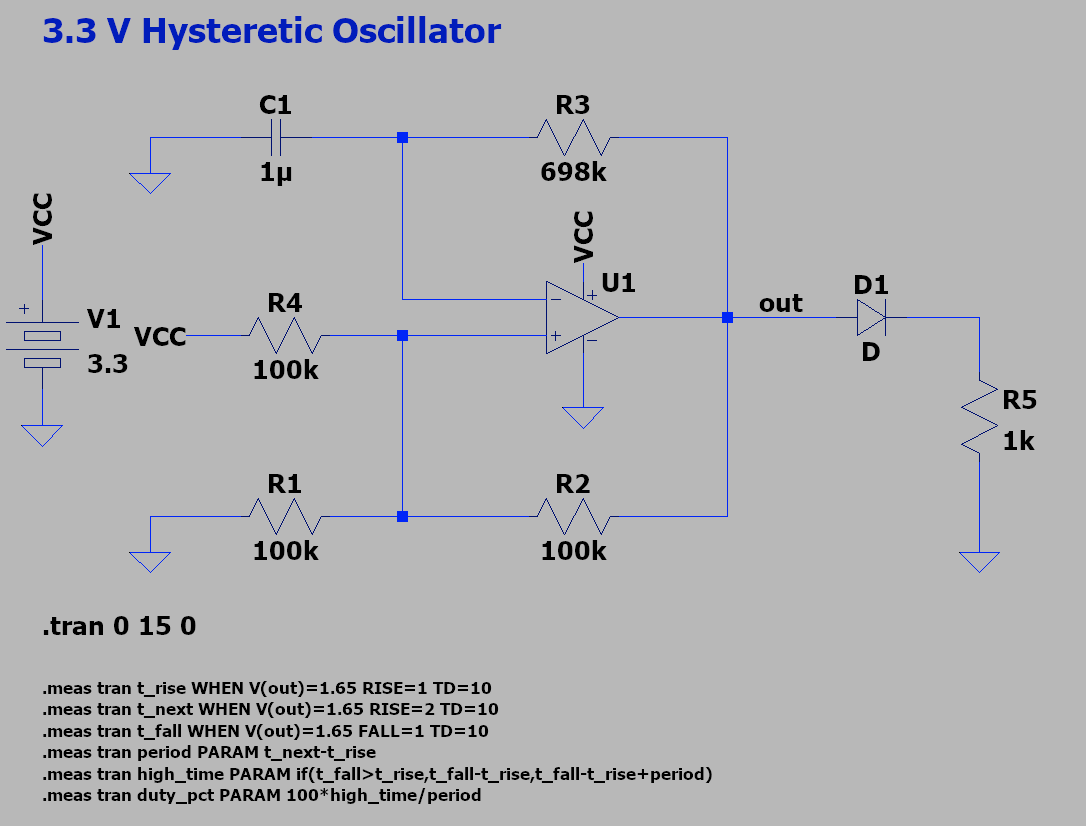
\includegraphics[width=0.75\linewidth]{ltspice-schematic.png}
  \caption{LTspice schematic with \texttt{.meas} statements for period and
  duty cycle.}
  \label{fig:ltspice-sch}
\end{figure}

\Cref{fig:ltspice-plot} shows the output. The simulation reports a period
of \qty{0.963}{\s} and a duty cycle of \qty{50.2}{\percent}, within
\qty{0.5}{\percent} of the prediction. The output sits at \qty{1.65}{\volt}
for the first few seconds because the simulation starts with both op-amp
inputs at exactly the same voltage and there is no noise to tip it one way;
a real circuit starts immediately.

\begin{figure}[H]
  \centering
  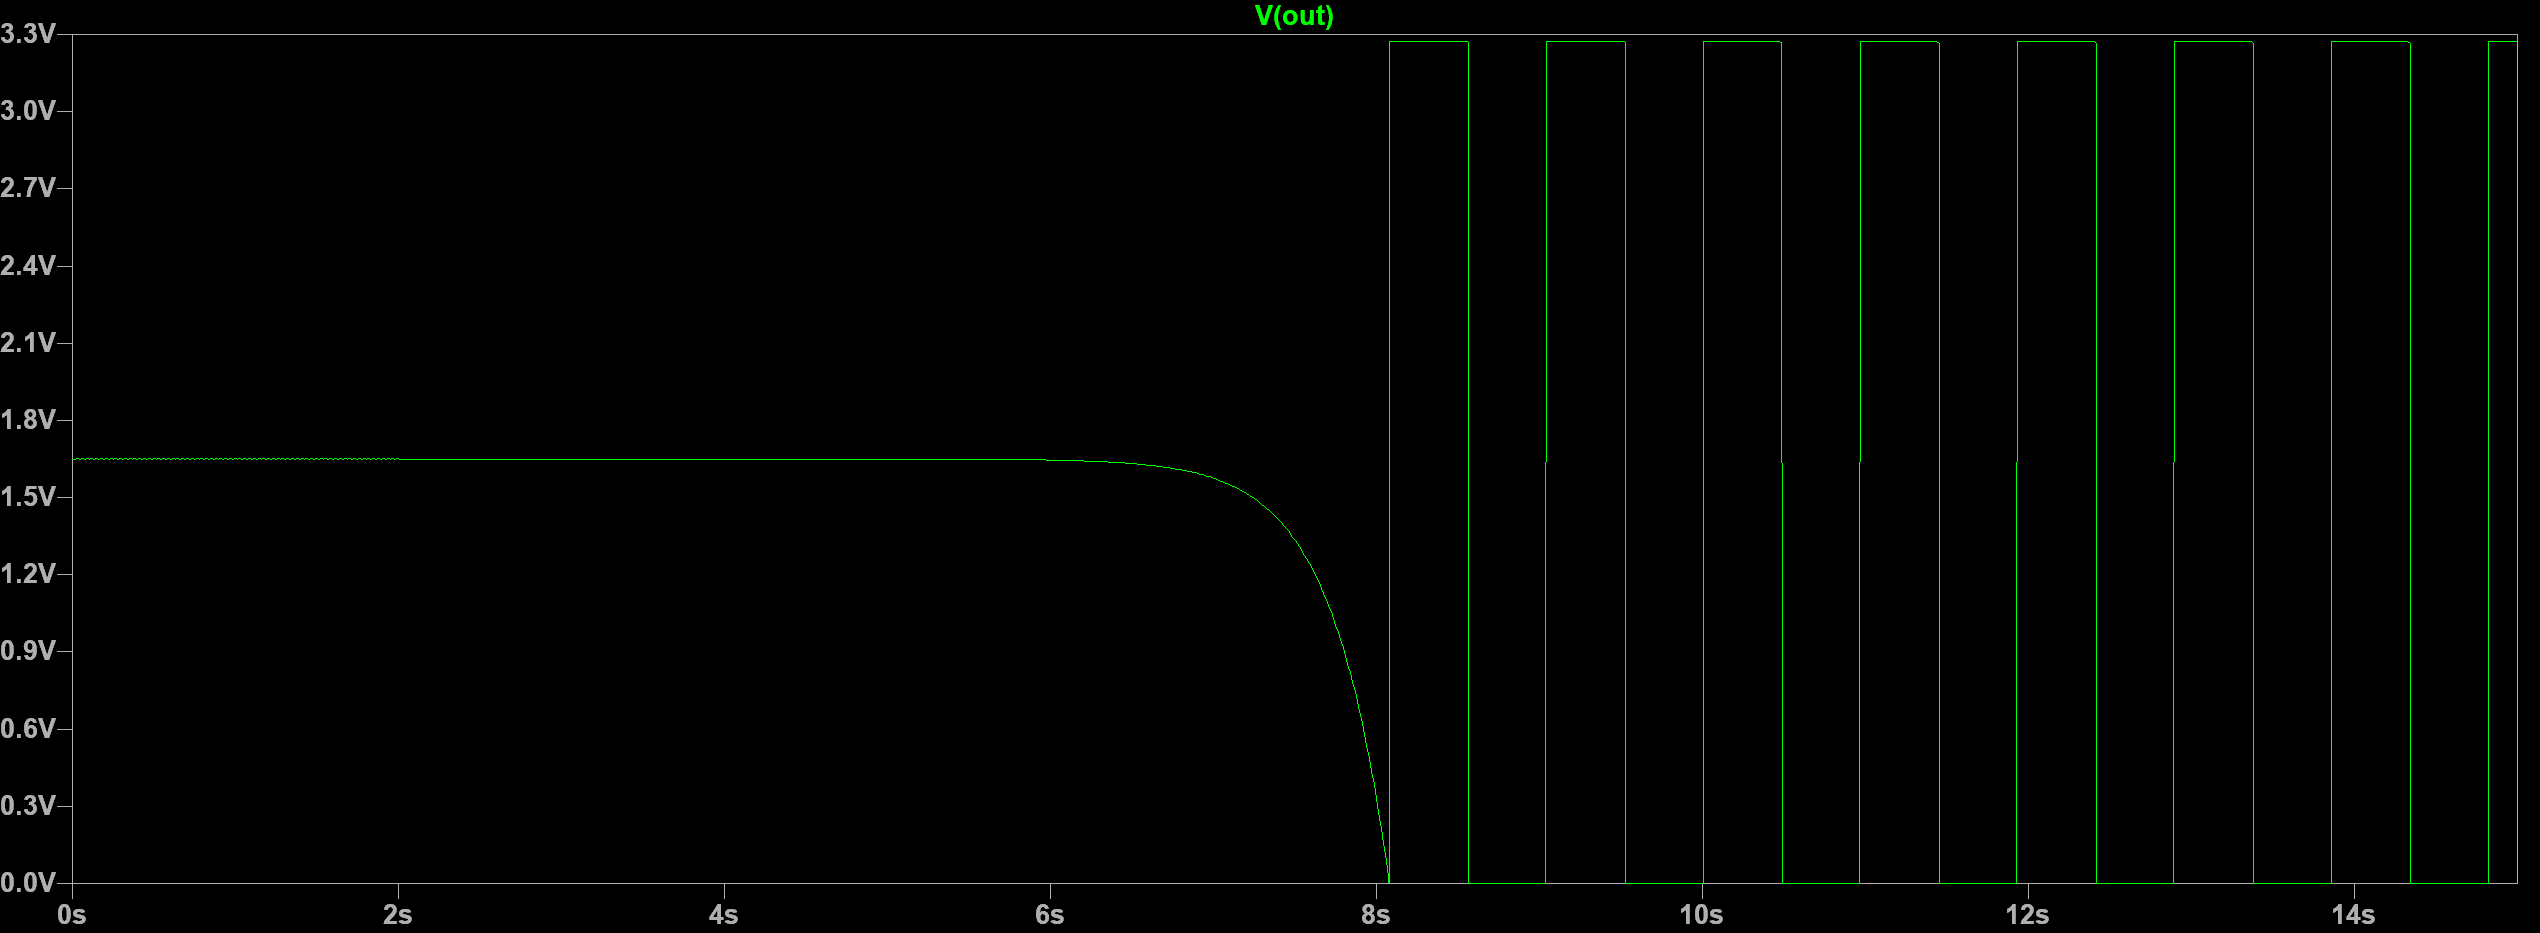
\includegraphics[width=0.97\linewidth]{ltspice-plot.png}
  \caption{Simulated output voltage.}
  \label{fig:ltspice-plot}
\end{figure}

\section{Bill of Materials}
\label{sec:bom}
All parts are drawn from the course spreadsheet. Reference designators
match the schematic in \cref{fig:schematic}.

\begin{table}[H]
  \centering
  \small
  \begin{tabularx}{\linewidth}{@{}l>{\raggedright\arraybackslash}Xcll>{\raggedright\arraybackslash}X@{}}
    \toprule
    Ref. des. & Description & Qty & Package & Mfr.\ part \# & Digi-Key \# \\
    \midrule
    J1        & USB-A plug, right angle, through-hole & 1 & --       & 0480370001         & WM17117-ND \\
    U1        & Op-amp, \qty{10}{\MHz} RRO, single    & 1 & SOT-23-5 & MCP6021T-E/OT      & MCP6021T-E/OTCT-ND \\
    U2        & LDO, \qty{3.3}{\volt}, \qty{250}{\mA} & 1 & SOT-23-3 & MCP1702T-3302E/CB  & MCP1702T-3302E/CBCT-ND \\
    D1        & LED, red, clear                       & 1 & 0805     & LTST-C171KRKT      & 160-1427-1-ND \\
    C1, C2, C5 & \qty{100}{\nano\farad} X7R \qty{50}{\volt} \qty{5}{\percent} & 3 & 0603 & CC0603JRX7R9BB104 & 311-1779-1-ND \\
    C3        & \qty{1}{\micro\farad} X7R \qty{25}{\volt} \qty{10}{\percent}  & 1 & 0603 & C0603C105K3RACTU   & 399-7376-1-ND \\
    C4        & \qty{10}{\micro\farad} X5R \qty{16}{\volt} \qty{10}{\percent} & 1 & 0603 & GRT188R61C106KE13D & 490-12317-1-ND \\
    R1, R2, R4 & \qty{100}{\kilo\ohm} \qty{1}{\percent} & 3 & 0603 & RC0603FR-07100KL   & 311-100KHRCT-ND \\
    R3        & \qty{3.01}{\mega\ohm} \qty{1}{\percent}  & 1 & 0603 & RC0603FR-073M01L   & 311-3.01MHRCT-ND \\
    R5        & \qty{1}{\kilo\ohm} \qty{1}{\percent}     & 1 & 0603 & RC0603FR-071KL     & 311-1.00KHRCT-ND \\
    R6        & \qty{604}{\kilo\ohm} \qty{1}{\percent}   & 1 & 0603 & RC0603FR-07604KL   & 311-604KHRCT-ND \\
    \bottomrule
  \end{tabularx}
  \caption{Bill of materials (15 components, 11 line items).}
  \label{tab:bom}
\end{table}

\section{PCB Layout}
\label{sec:pcb}
All components are on the top layer. Signals are routed on top and the bottom layer is a solid ground
pour, with a via at each ground pad. The USB connector sits on the bottom
edge with the regulator and its capacitors right behind it, the op-amp is
in the center with its bypass capacitor beside its supply pin, and the
timing parts are grouped together next to it. The LED is at the top edge
so it is visible when plugged in. \Cref{tab:layout} summarizes the layout
against the design rules; DRC passes with no violations.

\begin{figure}[H]
  \centering
  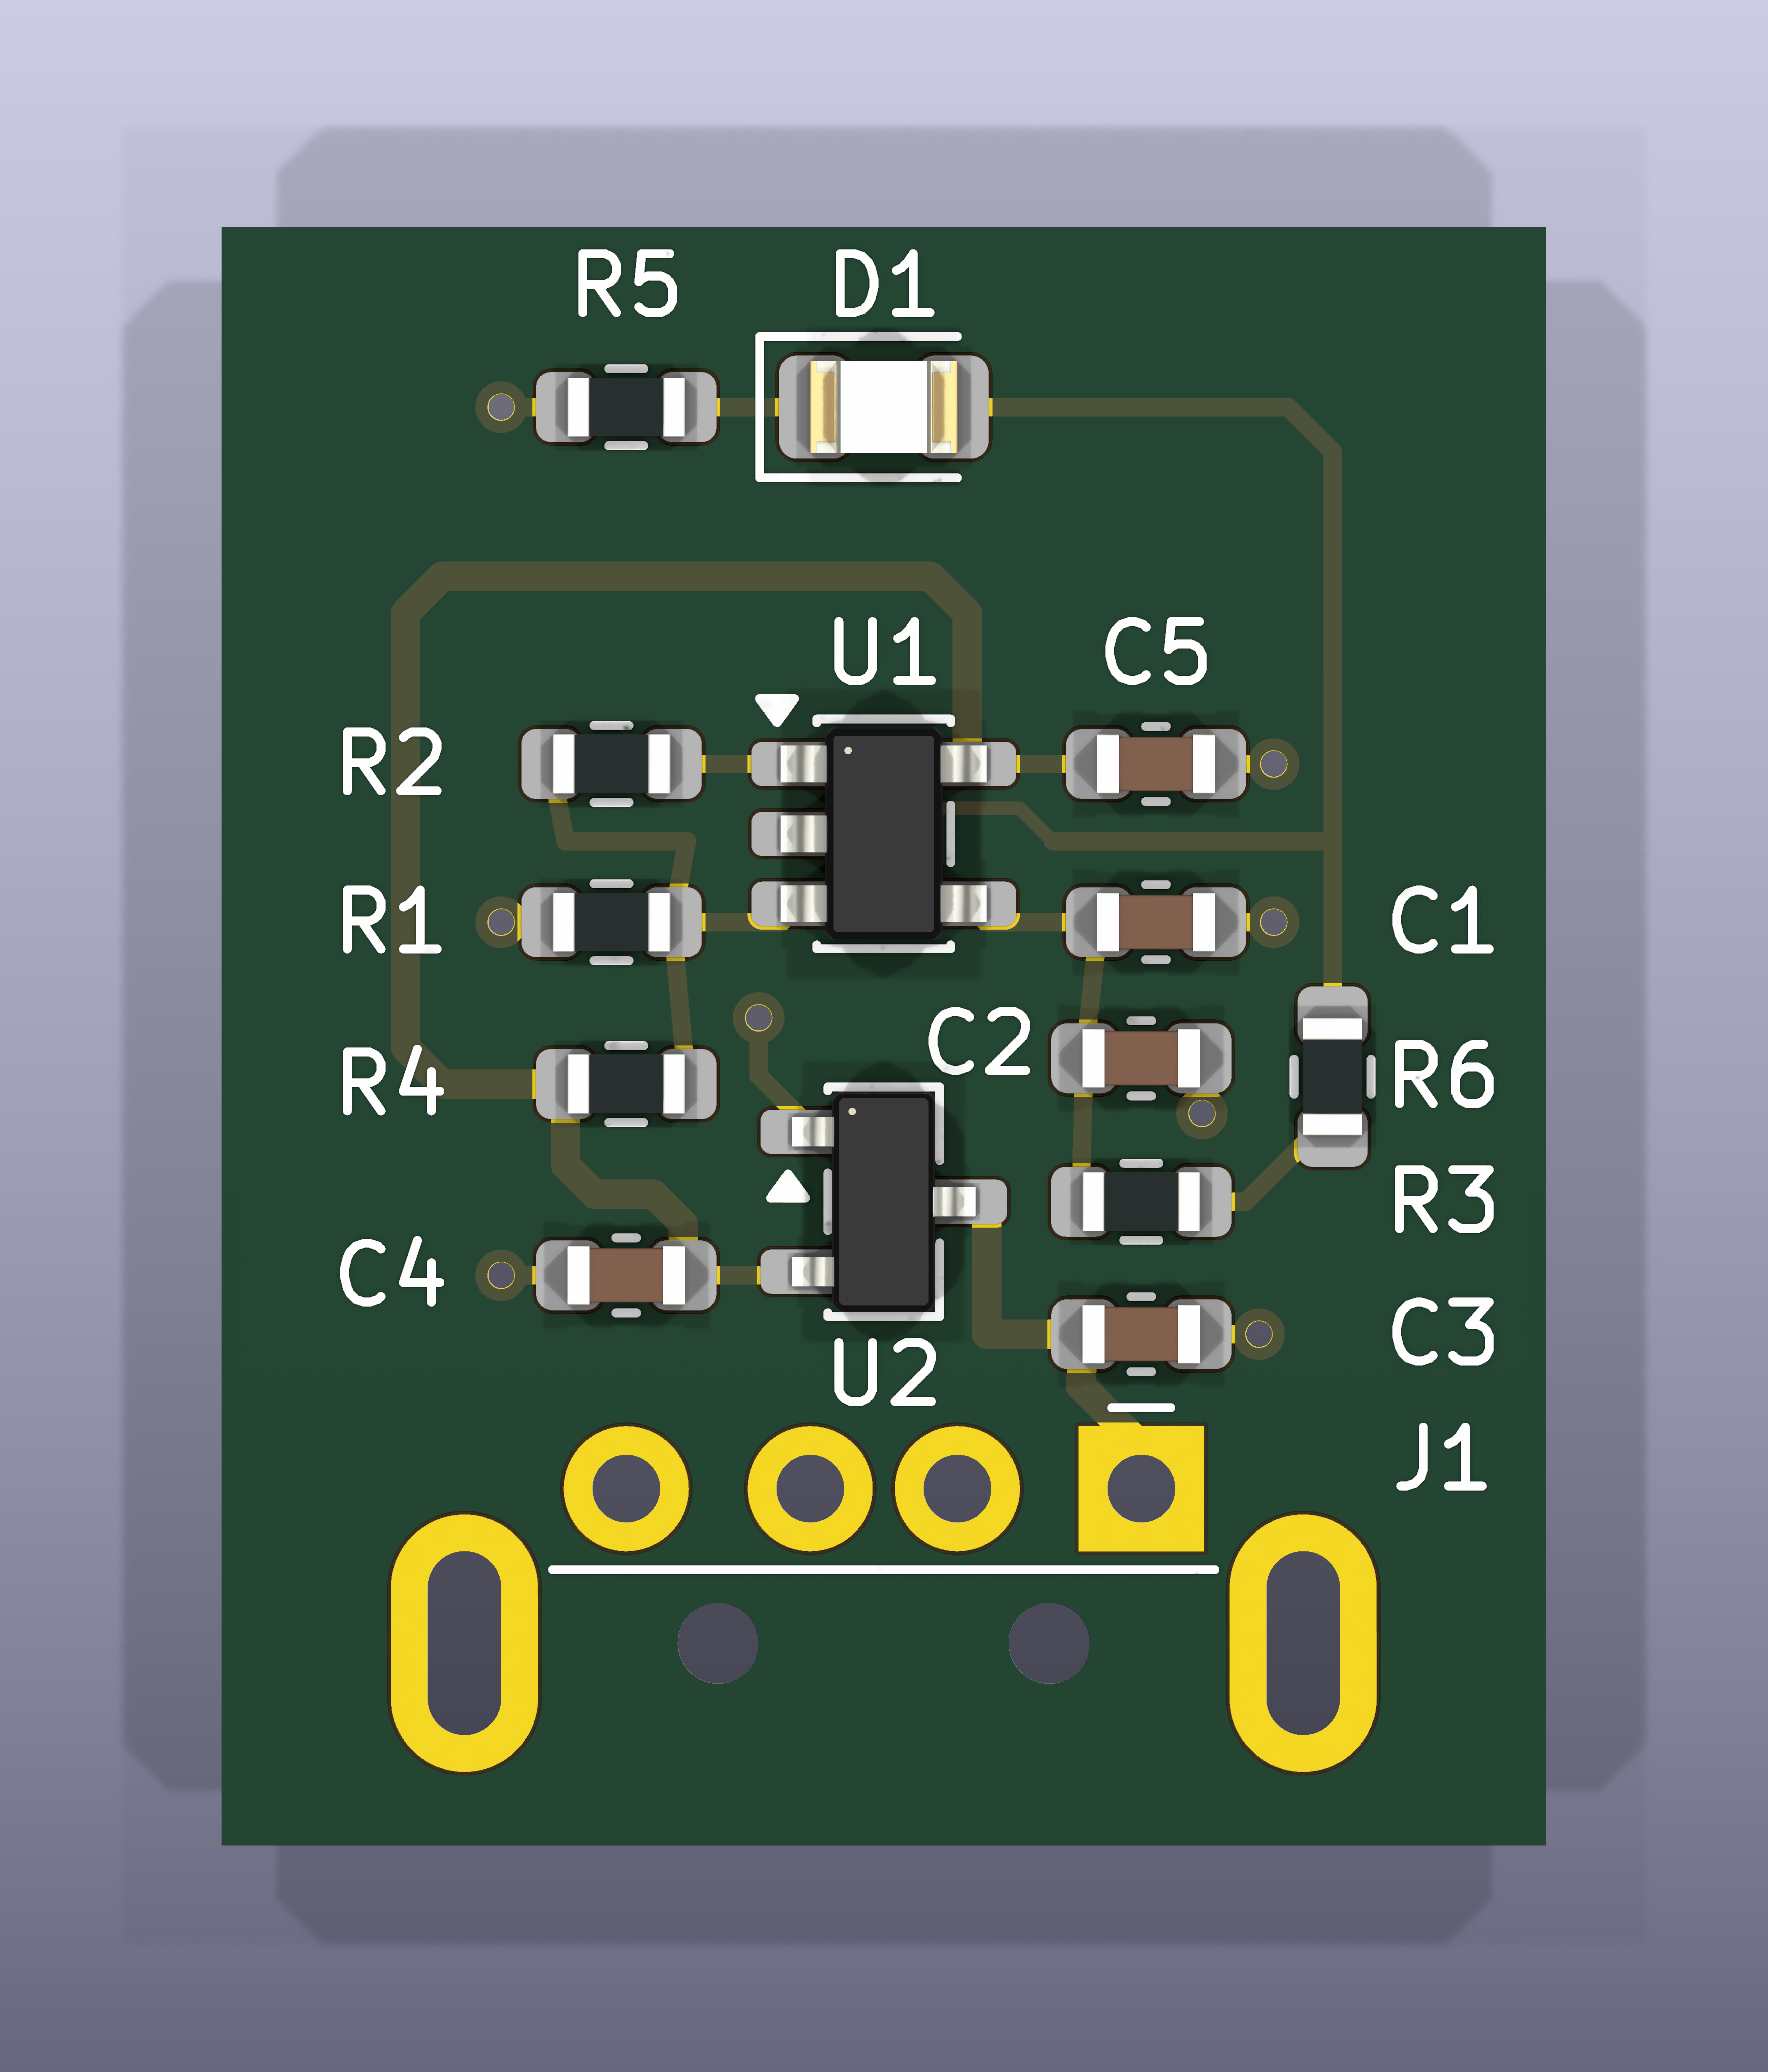
\includegraphics[width=0.4\linewidth]{pcb-top.png}\hspace{0.06\linewidth}
  
\includegraphics[width=0.4\linewidth]{pcb-bottom.png}
  \caption{3D render of the board: top side with components (left) and
  bottom ground pour (right).}
  \label{fig:pcb}
\end{figure}

\begin{table}[H]
  \centering
  \begin{tabular}{@{}lS[table-format=3.2]@{}}
    \toprule
    Metric & {Value} \\
    \midrule
    Board width (\unit{\mm})    & 18 \\
    Board height (\unit{\mm})   & 22 \\
    Bounding-box area (\unit{\mm\squared}) & 396 \\
    Min.\ trace width used (mil) & 7.09 \\
    Via count                    & 9 \\
    DRC violations               & 0 \\
    \bottomrule
  \end{tabular}
  \caption{Layout summary.}
  \label{tab:layout}
\end{table}

\section{Design Files}
\label{sec:files}
All design files, including the KiCad project, LTspice simulation, and this
report, are in the GitHub repository at
\url{https://github.com/flipper-slipper/eclectronics-fall-2026}.

\end{document}
